\documentclass{cshwk}

\usepackage{tikz}
\usetikzlibrary{arrows.meta, positioning}

\begin{document}

\title{HW \#2, Chapter 2}

\maketitle
\section*{Problem 3. Chapter 2 SECTION 2.2-2.5 R16.}

Suppose Alice, with a Web-based e-mail account (such as Hotmail or Gmail), sends a message to Bob, who accesses his mail from his mail server using IMAP. Discuss how the message gets from Alice’s host to Bob’s host. Be sure to list the series of application-layer protocols that are used to move the message between the two hosts.

\subsection*{Answer}


\subsubsection*{Stages of Email Transmission}

\begin{enumerate}
    \item \textbf{From Alice's Web Browser to Her Email Provider's Web Server}
    \begin{itemize}
        \item \textbf{Email Composition:} Alice composes an email using the web interface of her email provider (e.g., Gmail) in her web browser.
        \item \textbf{HTTPS Protocol:} Upon clicking "Send," the email is transmitted from her browser to her email provider's web server using \textbf{HTTPS} (HTTP over TLS/SSL), ensuring secure communication.
        \item \textbf{Server Processing:} The web server processes the request and forwards the email to the email provider's outgoing mail server.
    \end{itemize}
    
    \item \textbf{Between Mail Servers (Alice's Mail Server to Bob's Mail Server)}
    \begin{itemize}
        \item \textbf{SMTP Protocol:} The outgoing mail server uses \textbf{SMTP} (Simple Mail Transfer Protocol) to send the email to Bob's mail server.
        \item \textbf{DNS Lookup:} Alice's mail server performs a DNS query to find the MX (Mail Exchange) records for Bob's domain to identify his mail server.
        \item \textbf{Email Transmission:} The email is transmitted over the Internet from Alice's mail server to Bob's mail server using SMTP.
    \end{itemize}
    
    \item \textbf{From Bob's Mail Server to Bob's Mail Client}
    \begin{itemize}
        \item \textbf{Email Storage:} Bob's mail server stores the received email in his mailbox.
        \item \textbf{IMAP Protocol:} Bob's email client retrieves the email from the server using \textbf{IMAP} (Internet Message Access Protocol).
        \item \textbf{Secure Retrieval (Optional):} If security is enabled, \textbf{IMAPS} (IMAP over SSL/TLS) is used to encrypt the communication between Bob's client and mail server.
    \end{itemize}
\end{enumerate}

\subsubsection*{Application-Layer Protocols Used}

\begin{itemize}
    \item \textbf{HTTPS (HTTP over TLS/SSL):} Between Alice's web browser and her email provider's web server.
    \item \textbf{SMTP (Simple Mail Transfer Protocol):} Between Alice's mail server and Bob's mail server.
    \item \textbf{IMAP (Internet Message Access Protocol):} Between Bob's mail server and his email client.
\end{itemize}

\subsubsection*{Illustrative Diagram}

\begin{figure}[h!]
    \centering
    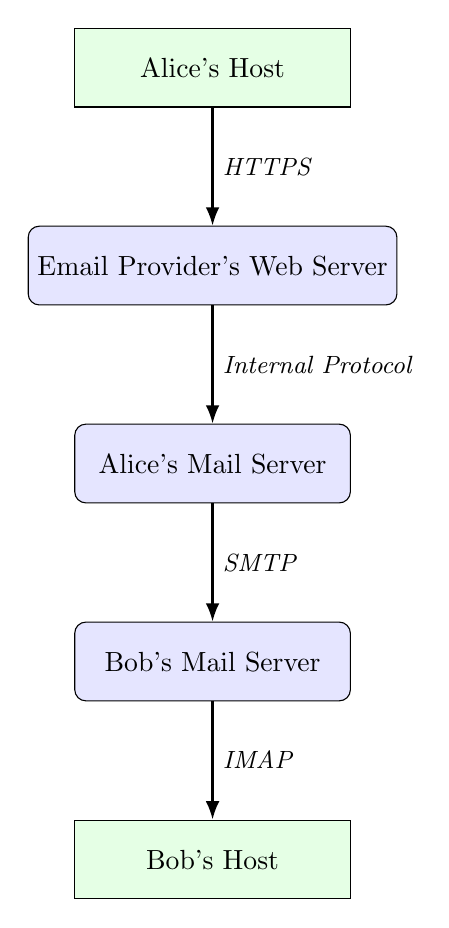
\begin{tikzpicture}[
        server/.style={rectangle, draw, rounded corners, fill=blue!10, minimum width=3.5cm, minimum height=1cm},
        client/.style={rectangle, draw, fill=green!10, minimum width=3.5cm, minimum height=1cm},
        protocol/.style={font=\small\itshape},
        arrow/.style={-Latex, thick},
        node distance=1.5cm,
        ]
    
        % Nodes
        \node[client] (AliceHost) {Alice's Host};
        \node[server, below=of AliceHost] (AliceWebServer) {Email Provider's Web Server};
        \node[server, below=of AliceWebServer] (AliceMailServer) {Alice's Mail Server};
        \node[server, below=of AliceMailServer] (BobMailServer) {Bob's Mail Server};
        \node[client, below=of BobMailServer] (BobHost) {Bob's Host};
    
        % Arrows and Protocols
        \draw[arrow] (AliceHost) -- node[right, protocol]{HTTPS} (AliceWebServer);
        \draw[arrow] (AliceWebServer) -- node[right, protocol]{Internal Protocol} (AliceMailServer);
        \draw[arrow] (AliceMailServer) -- node[right, protocol]{SMTP} (BobMailServer);
        \draw[arrow] (BobMailServer) -- node[right, protocol]{IMAP} (BobHost);
    
    \end{tikzpicture}
    \caption{Email Transmission from Alice to Bob}
\end{figure}

\noindent In the diagram:

\begin{itemize}
    \item \textbf{HTTPS} is used between Alice's host and her email provider's web server to securely send the email.
    \item \textbf{Internal Protocol} represents the communication within the email provider's system between the web server and the mail server (this could be SMTP or a proprietary protocol).
    \item \textbf{SMTP} is used between Alice's mail server and Bob's mail server to transfer the email over the Internet.
    \item \textbf{IMAP} is used between Bob's mail server and his host to retrieve the email.
\end{itemize}

\subsubsection*{Summary}

The email journey from Alice to Bob involves multiple application-layer protocols:

\begin{enumerate}
    \item Alice sends the email using \textbf{HTTPS} from her web browser to her email provider's web server.
    \item The email provider's mail server sends the email to Bob's mail server using \textbf{SMTP}.
    \item Bob retrieves the email from his mail server using \textbf{IMAP} on his email client.
\end{enumerate}

Each protocol plays a specific role in ensuring the email is securely composed, transmitted, and retrieved.

\end{document}
